\documentclass[tikz,border=3pt]{standalone}
\usepackage[utf8]{inputenc}
\usepackage[T1]{fontenc}
\usepackage{lmodern}
\renewcommand{\familydefault}{\sfdefault}
\usepackage{sansmath}\sansmath
\usepackage{chemfig}
\usepackage{pgfplots}\pgfplotsset{compat=1.18,/pgf/number format/use comma,/pgf/number format/1000 sep={.}}
\usetikzlibrary{arrows.meta,calc,positioning,decorations.pathmorphing,patterns}
% paleta del sitio
\definecolor{nar}{HTML}{E8680C}\definecolor{narc}{HTML}{FFB35C}\definecolor{hielo}{HTML}{FFF3E8}
\definecolor{tinta}{HTML}{1D1D1F}\definecolor{gris}{HTML}{6E6E73}\definecolor{lila}{HTML}{7C5CF0}
\definecolor{azul}{HTML}{2F6FD6}\definecolor{menta}{HTML}{17A673}\definecolor{coral}{HTML}{E8342A}
\begin{document}
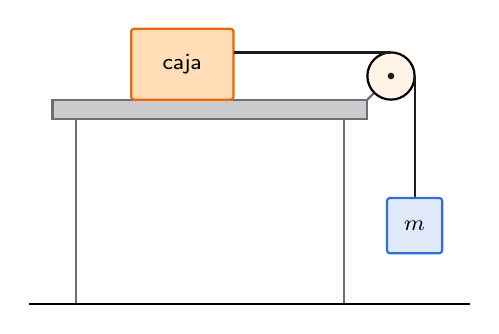
\begin{tikzpicture}[font=\footnotesize,>={Stealth[length=2.4mm]}]
% mesa
\fill[gris!35] (0,-0.25) rectangle (4,0);
\draw[thick,gris] (0,-0.25) rectangle (4,0);
\draw[thick,gris] (0.3,-0.25) -- (0.3,-2.6) (3.7,-0.25) -- (3.7,-2.6);
\draw[thick] (-0.3,-2.6) -- (5.3,-2.6);
% caja
\draw[thick,draw=nar,fill=narc!45,rounded corners=1pt] (1.0,0) rectangle (2.3,0.9);
\node at (1.65,0.45) {caja};
% polea
\draw[thick,gris] (4,0) -- (4.3,0.3);
\draw[thick,fill=hielo] (4.3,0.3) circle (0.3);
\fill[tinta] (4.3,0.3) circle (1.2pt);
% cuerda
\draw[thick,tinta] (2.3,0.6) -- (4.3,0.6);
\draw[thick,tinta] (4.6,0.3) -- (4.6,-1.25);
% cuerpo colgante
\draw[thick,draw=azul,fill=azul!15,rounded corners=1pt] (4.25,-1.25) rectangle (4.95,-1.95);
\node at (4.6,-1.6) {$m$};
\end{tikzpicture}
\end{document}
